\chapter{Ghidul utilizatorului}\label{ch:5interfataUtilizator}

	În acest capitol voi descrie felul în care utilizatorul poate să interacționeze cu aplicația web, iar în cele din urmă voi prezenta una dintre optimizările esențiale aduse sistemului.

\section{Interfața cu utilizatorul}

	Toate paginile au aceeasi structură: antet, meniu de navigare și secțiune pentru afișarea conținutului.

	Antet-ul conține o imagine și un logo.
	
	Bara de navigare se adapteaza in funcție de rolul utilizatorului. Unele butoane devin, sau nu, disponibile.
	
	Secțiunea de conținut, aceasta este diferita la fiecare pagină in parte.
	
\vspace{1em}

	Pagina \textit{Login} – structura acestei pagini este diferită față de celelalte. Conține un div cu imagine de fundal și un formular care face posibilă conectarea la aplicația web. Se vor introduce credențialele în câmpurile puse la dispoziție, iar după validarea acestora, se face redirecționarea la pagina principală.

\begin{figure}[H]
   	\centering
    	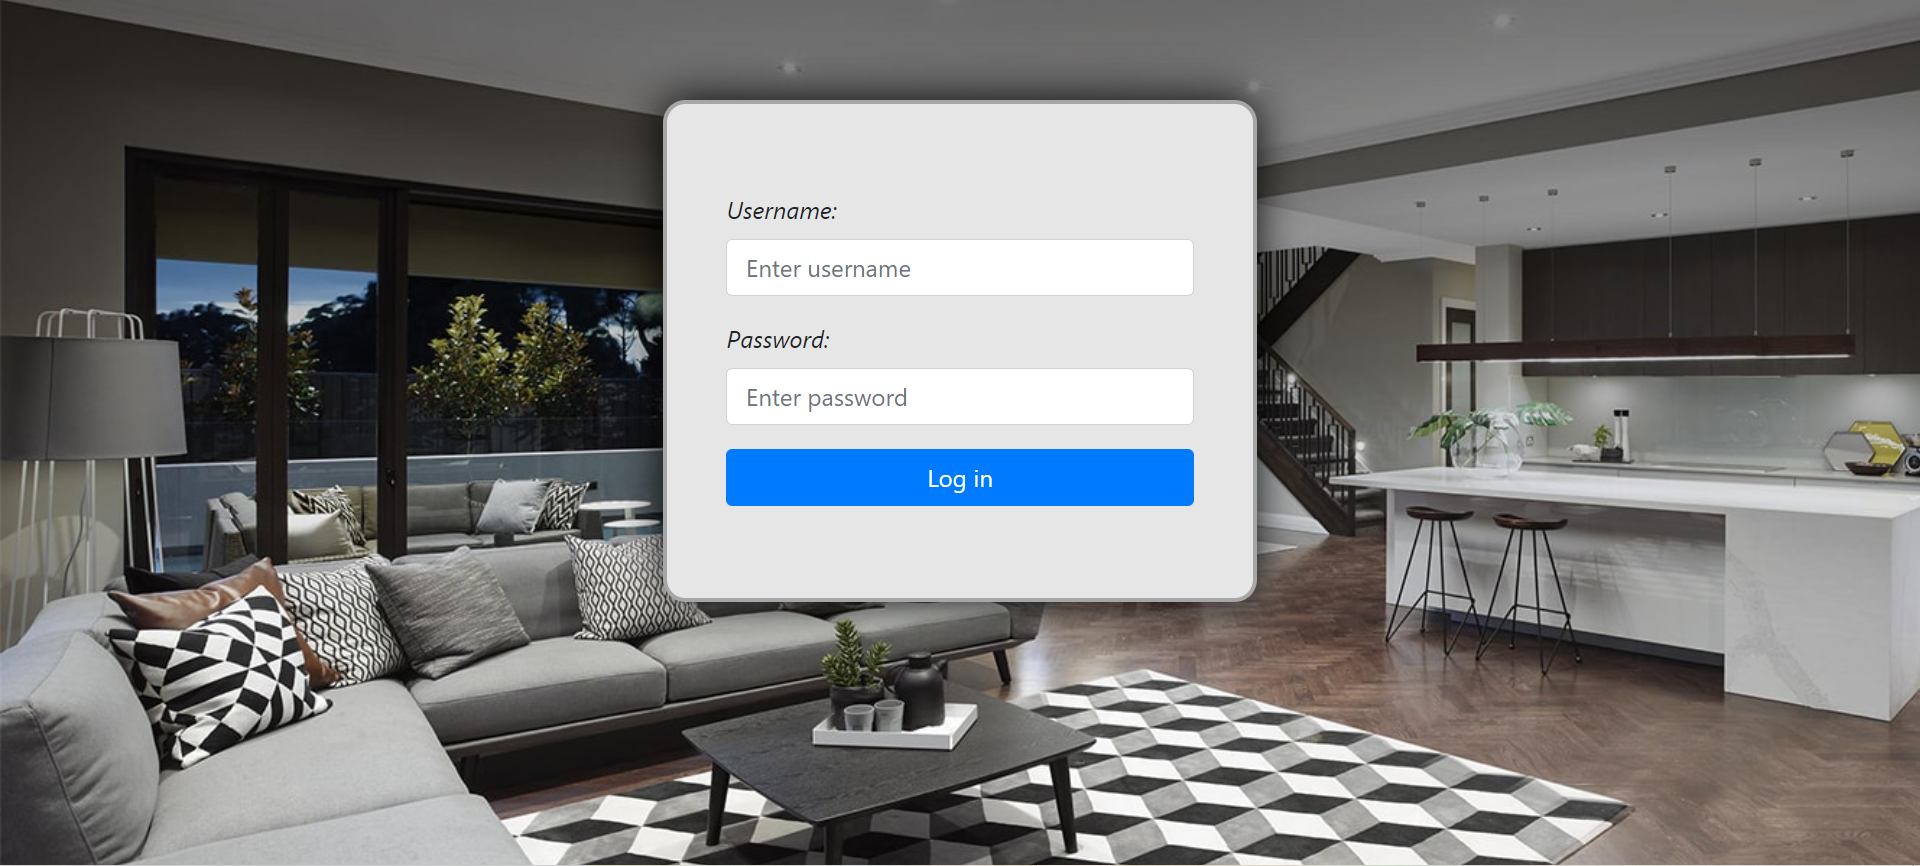
\includegraphics[width=0.8\textwidth]{Login.png}
	\caption{Pagina de conectare}
\end{figure}

	Pagina \textit{Home} – este accesibilă pentru toți utilizatorii și permite monitorizarea si setarea temperaturii. Modificarea valorii temperaturii se face prin intermediul cursoarelor prezente pe pagină. Butonul \textit{Set temperature} va determina actualizarea valorilor în baza de date. Pentru a putea modifica modul de operare al sistemului, se actionează butonul din dreptul etichetei \textit{Switch intervals on/off}. Dacă modul de operare pe intervale orare este activat, alăturat butonului \textit{on/off}, va mai apărea un buton ce va permite redirecționarea la o nouă pagină unde se pot seta intervalele orare și temperaturile.

\begin{figure}[H]
   	\centering
    	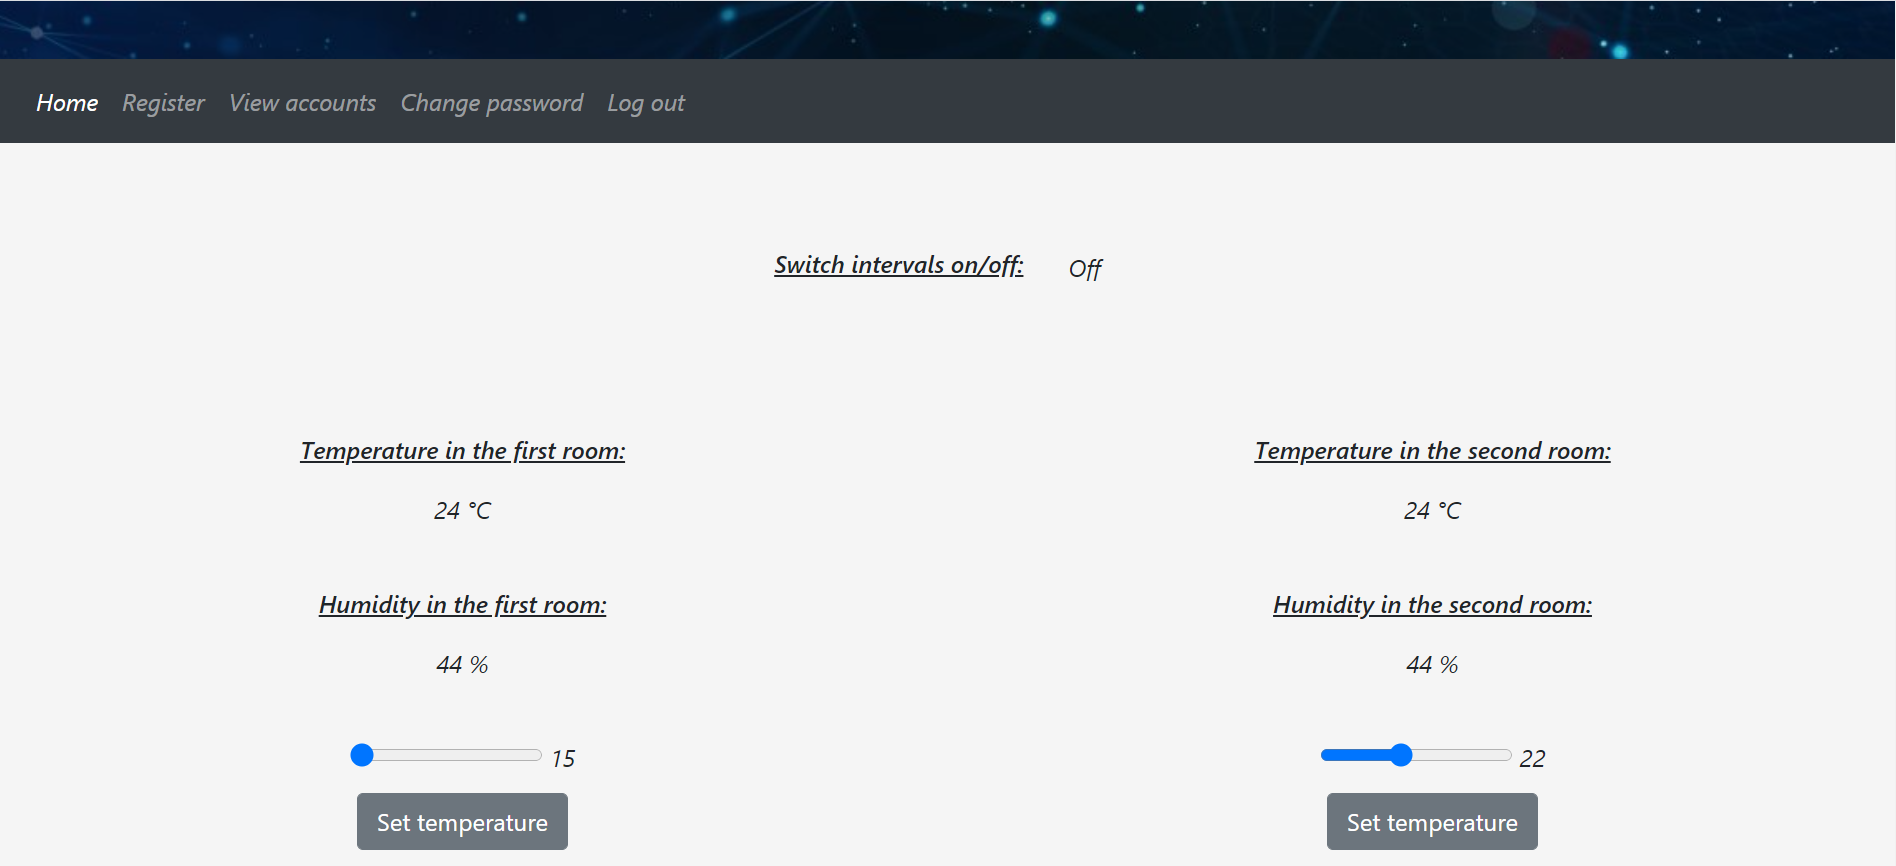
\includegraphics[width=0.8\textwidth]{Home.png}
	\caption{Pagina de setare a temperaturilor}
\end{figure}

	Pagina pentru setarea unui program de funcționare este disponibilă doar în modul automat. Fiecare câmp creat pentru introducerea valorii temperaturii conține o etichetă ce indică intervalul pentru care este valabilă temperatura setată. De exemplu, câmpul cu eticheta \textit{Temperature 1} va conține valoarea temperaturii ce se aplică primului interval orar. Un interval orar are ca și capete două valori de timp setate în câmpuri consecutive.  

\begin{figure}[H]
   	\centering
    	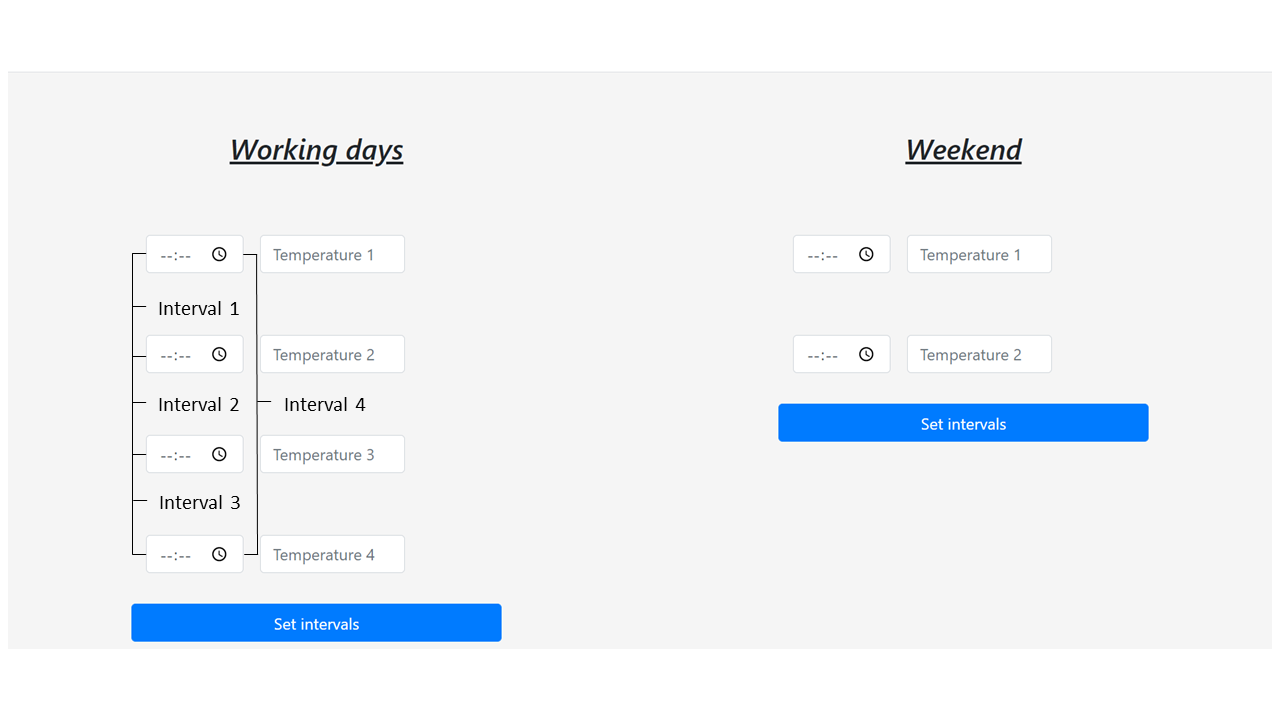
\includegraphics[width=0.8\textwidth]{SetIntervals.png}
	\caption{Pagina de setare a programului de funcționare}
\end{figure}

	Pagina \textit{Register} – accesibilă doar pentru administrator și face posibilă crearea de noi conturi. Formularul permite introducerea credențialelor pentru contul creat, iar câmpul \textit{Give admin privileges?} este utilizat pentru setarea drepturilor.

\begin{figure}[H]
   	\centering
    	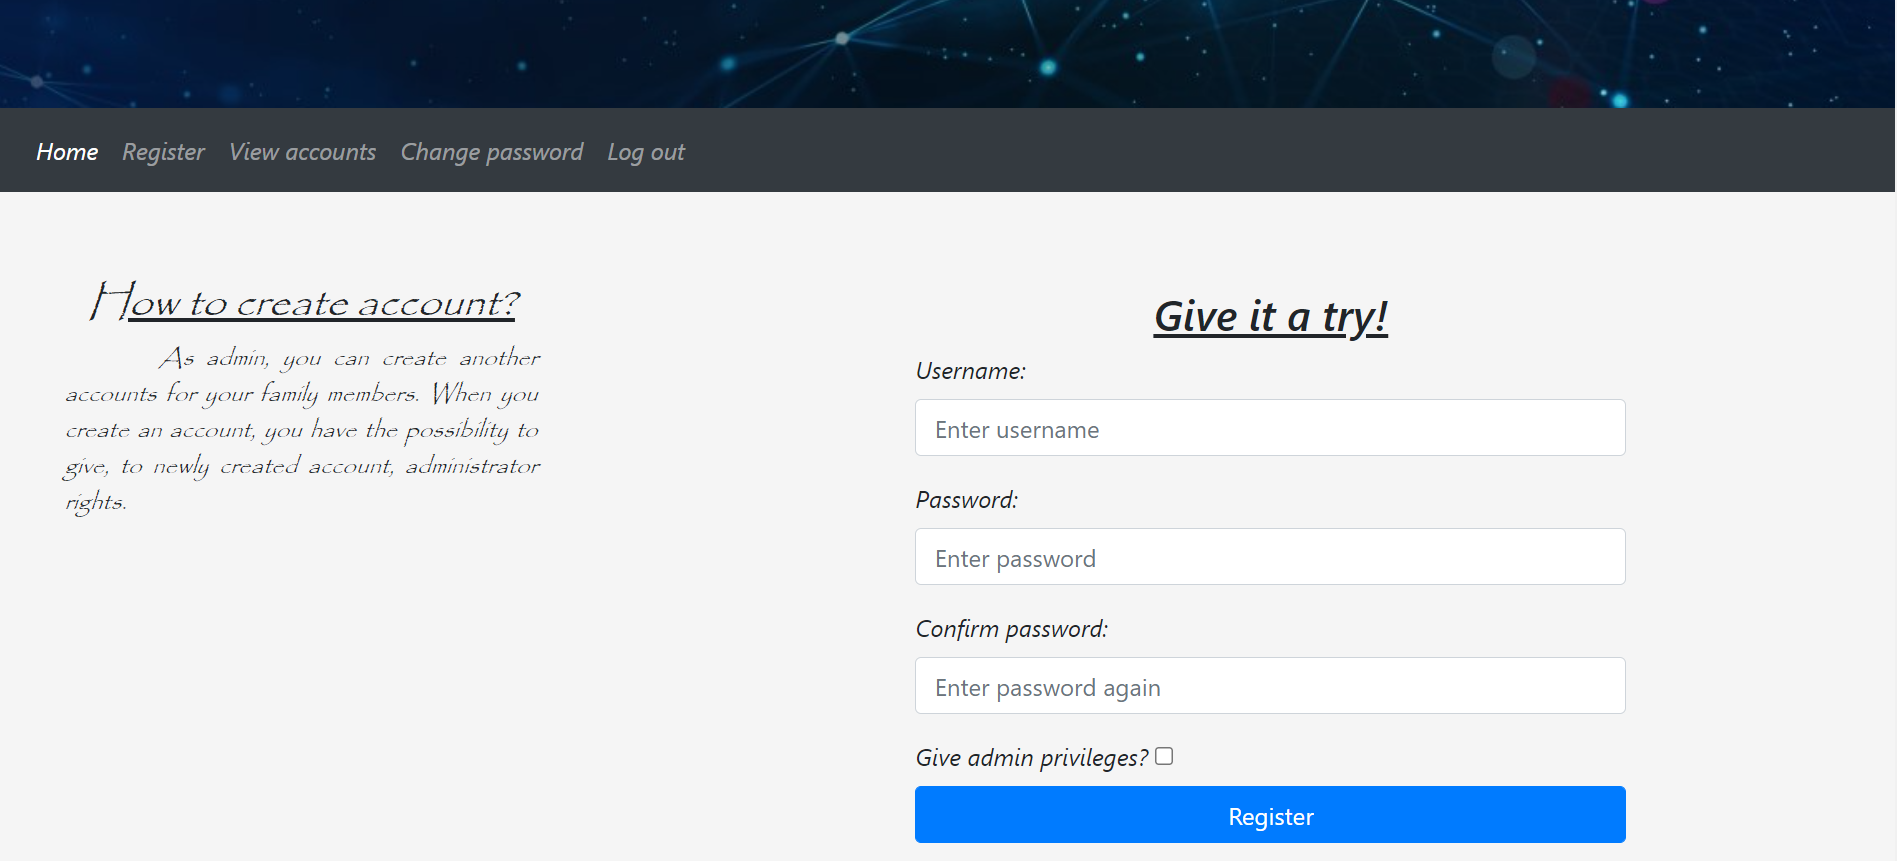
\includegraphics[width=0.8\textwidth]{Register.png}
	\caption{Pagina creare cont}
\end{figure}

	Pagina \textit{View accounts} – este accesibilă doar de către administratori, oferind posibilitatea de a modifica drepturile utilizatorilor și de a șterge alte conturi. De asemenea, se afișează o listă cu toți utilizatorii, împreună cu drepturile acestora.

\begin{figure}[H]
   	\centering
    	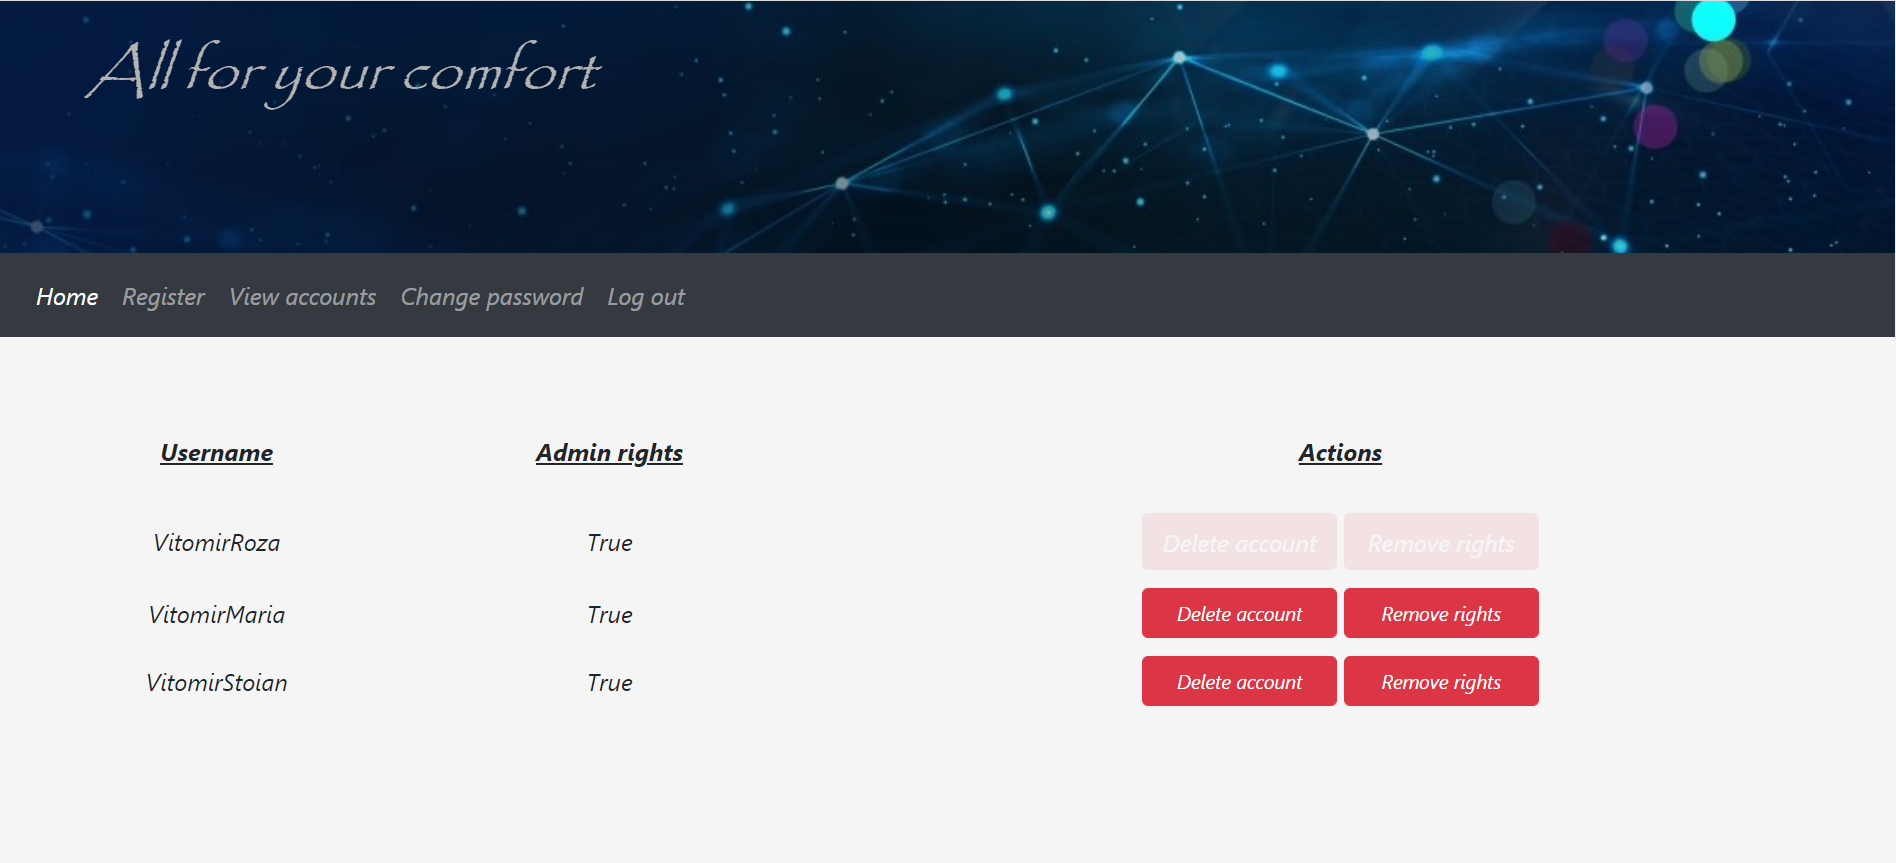
\includegraphics[width=0.8\textwidth]{ViewAccounts.png}
	\caption{Pagina vizualizare conturi}
\end{figure}

	Pagina \textit{Change password} – permite modificarea parolei pentru fiecare utilizator. Câmpul \textit{Current password} trebuie completat cu parola actuală a contului curent, iar câmpurile \textit{New password} și \textit{Confirm new password} vor conține noua parolă, respectiv confirmarea noii parole.

\begin{figure}[H]
   	\centering
    	\includegraphics[width=0.8\textwidth]{ChangePassword.png}
	\caption{Pagina schimbare parolă}
\end{figure}

\section{Optimizare}

	În acest subcapitol voi prezenta una din optimizările pe care a fost necesar să o implementez pentru a reduce consumul de date. Resursele pe care baza de date le pune la dispoziție sunt limitate. Prin urmare, există și o limitare în ceea ce privește capacitatea datelor descărcate.

	Primele versiuni de cod pentru modulul WiFi făceau ca la fiecare iterație a instrucțiunii repetitive \textit{loop} să se citească valorile temperaturilor și intervalelor din baza de date. Motiv pentru care, consumul de date era mare.  În figura următoare, este ilustrată cantitatea de date citite în decursul a unei jumătăți de oră de funcționare.
 
\begin{figure}[H]
   	\centering
    	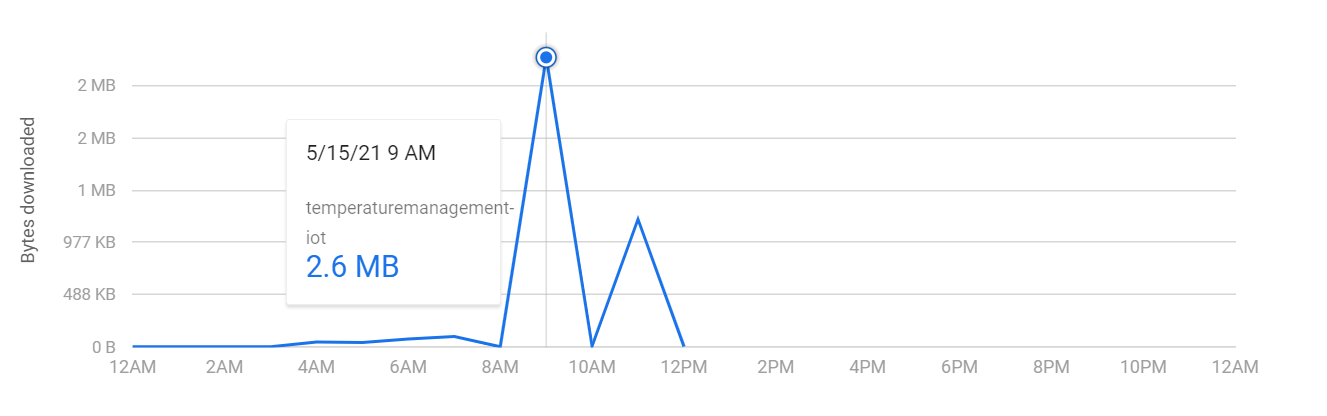
\includegraphics[width=0.8\textwidth]{FaraOptimizare.png}
	\caption{Versiunea de cod neoptimizată}
\end{figure}

	Pentru a renunța la acest comportament, a fost necesară modificarea implementării codului. Astfel, citirile se vor realiza doar în momentul în care se modifică valorile din baza de date. În figura atașată, se ilustrează consumul de date în urma funcționării timp de jumătate de oră cu noul cod. În acest timp, pentru a face o simulare cât mai complexă, am setat diferite valori ale temperaturii prin intermediul aplicației web. 

\begin{figure}[H]
   	\centering
    	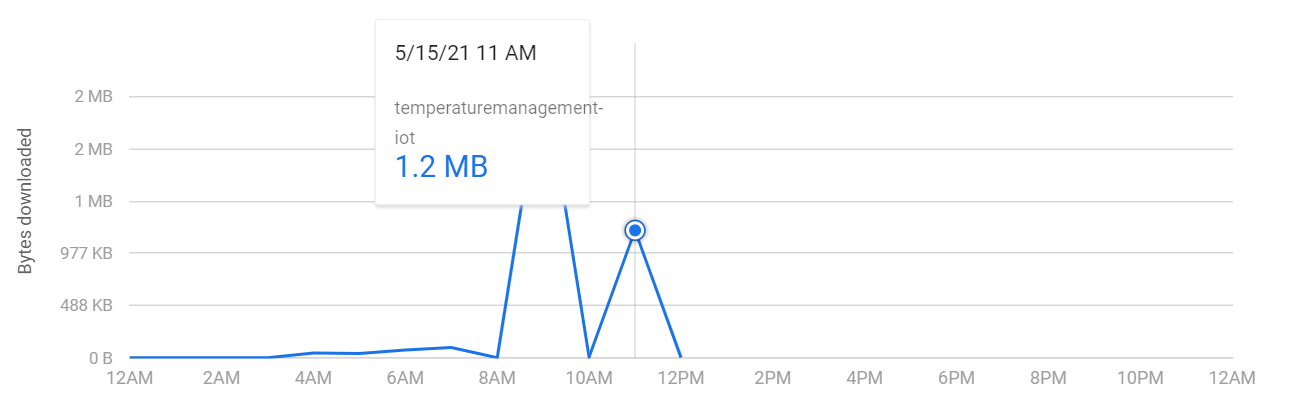
\includegraphics[width=0.8\textwidth]{CuOptimizare.png}
	\caption{Versiunea de cod optimizată}
\end{figure}

	În urma acestui experiment, se poate observa o scădere considerabilă a consumului de date, fapt ce face posibilă funcționarea sistemului în mod continuu. 

